\chapter{A tervezés részletes leírása és szoftverarchitektúrája}
\label{chap:tervezes}

A specifikációban rögzített funkcionális és nem-funkcionális követelmények elérése érdekében a szimulációs keretrendszer tervezése során kiemelt figyelmet fordítottam a modern szoftvertechnológiai minták alkalmazására.

Az MSc szintű diplomaterv célkitűzéseinek megfelelően a tervezés fókuszában a monolitikus struktúrák felbontása, a tiszta komponens-alapú aggregáció, valamint a skálázhatóságot garantáló eseményvezérelt működés állt.

Ez a fejezet részletesen bemutatja a rendszer szoftverarchitektúráját, az ágensek belső dekompozícióját és az alkalmazott kommunikációs modelleket a megvalósított forráskód alapján.

% 4.1
%~~~~~~~~~~~~~~~~~~~~~~~~~~~~~~~~~~~~~~~~~~~~~~~~~~~~~~~~~~~~~~~~~~~~~~~~~~~~~~~~~~~~~~
\section{Architekturális áttekintés}
\label{sec:architektura}

A projekt fejlesztése során a legfőbb szoftvertechnológiai kihívást az ágensek belső felépítésének menedzselése jelentette. A játékmotor-fejlesztésben gyakran előforduló „Istenszerű osztály” (\textit{God Class}) antiminta elkerülése érdekében a rendszer egy hibrid, absztrakcióra és komponens-aggregációra épülő architektúrát kapott.

A hierarchia csúcsán a \texttt{MonoBehaviour}-ból származtatott absztrakt \texttt{Animal} osztály áll, amely nem közvetlenül implementálja a biológiai és fizikai funkciókat, hanem összefogja, konfigurálja és koordinálja a specializált részkomponenseket.

Az \texttt{Animal} ősosztály felelőssége a közös állapotváltozók, a térbeli referenciák, valamint a genotípushoz kapcsolódó alapvető tulajdonságok tárolása.

A tényleges működési logikát a finomabb granularitású komponensek valósítják meg:
\begin{enumerate}
    \item \textbf{Fiziológiai komponensek} - a belső biológiai szükségletek és az életciklus fenntartásáért felelős modulok gyűjteménye:
    \label{item:fiziologia_enum}
    \begin{itemize}
        \item \texttt{Age}: az egyed folyamatos öregedését és fiatalkori növekedését vezérli a \texttt{lifeSpan} és \texttt{adultSize} paraméterek alapján
        \item \texttt{Eat}: a \texttt{currentHunger} értékcsökkenését menedzseli, kritikus szintnél kiváltja az \texttt{OnHungerCritical} eseményt, illetve kezeli a táplálkozással járó érték és státusz változásokat, illetve frissítí a kapcsolódó \texttt{HungerBar} vizuális elemet
        \item \texttt{Drink}: az \texttt{Eat} komponenshez hasonlóan működik a \texttt{currentThirst} változó mentén, vízhiány esetén az \texttt{OnThirstCritical} triggerelésével
        \item \texttt{Rest}: a fáradtságot és a pihenési hajlandóságot szabályozza, úgy, hogy tesz egy valószínűségi alapú döntést, amivel pihenés állapotba kényszerítheti az ágenst
    \end{itemize}

    \item \textbf{Reprodukciós komponensek} - az evolúciós motor alapját képező, párválasztási és utódnemzési folyamatokat tömörítő réteg:
    \begin{itemize}
        \item \texttt{Mate}: kezeli a nemi érettséget, a párzási kényszer szintjét, a cooldown fázisokat, valamint az \texttt{IsAcceptable()} metódussal eldönti, hogy a kiszemelt partner vonzereje, az aktuális szükségletek mellett elegendő-e az elfogadáshoz
        \item \texttt{Reproduction}: kizárólag a nőstény egyedeknél aktív modul, sikeres párzás után menedzseli a terhességi időt, illetve kezeli az utódok világrahozatalát a szülők értékei alapján
    \end{itemize}

    \item \textbf{Interakciós és fizikai komponensek} - az ágens környezetbe ágyazottságát, térbeli helyváltoztatását és észlelését biztosító rendszerek:
    \begin{itemize}
        \item \texttt{Movement}: a fizikai helyváltoztatást valósítja meg az ágens állapota alapján, célirányos mozgás (\texttt{Move}) vagy menekülés (\texttt{Flee}) esetén 5x-ös rotációs sebesség-szorzót alkalmaz forduláshoz, a céltalan bolyongással szemben (\texttt{Wander})
        \item \texttt{Sensor}: a környezet folyamatos pásztázásáért felelős modul, dinamikusan kalkulálja a ragadozók észlelési esélyét a távolság, valamint a préda \texttt{camouflage} és \texttt{stealth} genetikai tulajdonságai alapján
        \item \texttt{Die}: az elhullás végpontja, a fizikai GameObject, valamint a hozzátartozó \texttt{destructibles} elemek memóriából való takarításáért felelős, illetve \texttt{DebugLoggerrel} regisztrálja az állat statisztikáit, és elhalálozás körülményeit
    \end{itemize}
\end{enumerate}

A kiterjeszthetőséget és az Open/Closed elv érvényesülését az absztrakt metódusok (például \texttt{getTargetLayerToMate()}) biztosítják. Ezek révén a specifikus fajok, mint a \texttt{Bunny} és a \texttt{Fox}, destruktív kódmódosítás nélkül, deklaratív módon határozzák meg a saját rétegmaszk-alapú interakcióikat a Unity \texttt{LayerMask} rendszerében:

\begin{lstlisting}[language=csh, caption={Nyulak esetén a célréteg kiválasztása}, label={lst:bunny_layer}]
public class Bunny : Animal, IEdible
{
    ...
    public override int getTargetLayerToMate()
    {
        return LayerMask.GetMask("Bunny");
    }
    ...
}
\end{lstlisting}

A környezeti elemek absztrakcióját az \texttt{IEdible} interfész biztosítja. Ez a tervezési mintázat lehetővé teszi, hogy a ragadozók és a növényevők egységesen kezeljék a táplálékforrásokat:

A \texttt{Plant} osztály és a préda szerepet betöltő \texttt{Bunny} osztály egyaránt implementálja az \texttt{IEdible} interfészt. Így amikor egy ágens táplálkozni szeretne, a \texttt{targetRef} entitáson keresztül közvetlenül eléri a metódusait (például a \texttt{nutrition} értéket, ami meghatározza, hogy az elfogyasztott egyed mennyivel fogja csökkenteni az állat éhségérzetét), függetlenül attól, hogy növényi vagy állati eredetű biomasszáról van szó:

\begin{lstlisting}[language=csh, caption={Polimorfikus táplálkozáskezelés az IEdible interfészen keresztül}, label={lst:edible_eating}]
public void Eating()
{
    if (animal.targetRef != null && animal.targetRef.TryGetComponent<IEdible>(out var edibleFood))
    {
        // Egységes tápérték lekérdezés forrástól függetlenül:
        currentHunger = Mathf.Min(currentHunger + edibleFood.getNutrition(), maxHunger);
        
        // Az célobjektum értesítése az elfogyasztásról:
        edibleFood.Consumed();

        // Táplálkozással kapcsolatos értékek visszaállítása default értékekre:
        animal.targetRef = null;
        animal.sensor.targetMask = LayerMask.GetMask("None");
    }
    else
    {
       // Ha esetleg a célobjektum már nem létezne, mert pl. megette más korábban, mint elértük volna, folytatjuk a keresést:
        (animal.status, animal.prevStatus) = (animal.prevStatus, Status.WANDER);
        animal.targetRef = null;
    }
}
\end{lstlisting}

% 4.2
%~~~~~~~~~~~~~~~~~~~~~~~~~~~~~~~~~~~~~~~~~~~~~~~~~~~~~~~~~~~~~~~~~~~~~~~~~~~~~~~~~~~~~~
\section{Eseményvezérelt kommunikációs modell és az állapotgép frissítése}
\label{sec:esemenyvezerelt}

A szimuláció skálázhatóságát és valós idejű futását a leválasztott, eseményvezérelt kommunikációs architektúra garantálja, amely teljes mértékben felszámolja a képkocka-alapú folyamatos lekérdezést (\textit{polling}).

Az ágensek belső és külső eseményeinek szinkronizációjáért egy dedikált komponens, az \texttt{AnimalEventHandler} felel, amely hídként működik a fiziológiai komponensek (lásd: \ref{item:fiziologia_enum}. pontban) és az \texttt{Animal} központi állapotgépe között.

Az \texttt{Animal} osztály a \texttt{Subscribe()} metódusban iratkozik fel a részkomponensek által publikált C\# eseményekre (\texttt{Action}), amelyeket az \texttt{AnimalEventHandler} delegált metódusai kezelnek le. Ez a felépítés drasztikusan csökkenti a CPU terhelését, mivel a szimulált egyedek nem futtatnak felesleges ellenőrzéseket a Unity \texttt{Update()} ciklusában. Az állapotváltozások diszkrét, eseményalapú triggerelése a következő főbb láncolatokon keresztül zajlik:

\begin{itemize}
    \item \textbf{Fiziológiai krízishelyzetek:} Az \texttt{Eat} és \texttt{Drink} komponensek a \texttt{Step()} metódus periodikus lefutásakor ellenőrzik a belső értékeket. Amint az éhség vagy szomjúság eléri a kritikus szintet, kiváltódik az \texttt{OnHungerCritical} vagy \texttt{OnThirstCritical} esemény.

Az \texttt{AnimalEventHandler} ezen értesítések hatására azonnal átállítja az ágens \texttt{sensor.targetMask} értékét a megfelelő célobjektumra (például nyúl esetén \texttt{BunnyFood}, róka esetén \texttt{Bunny} lesz a réteg neve), és a státuszt \texttt{Status.SEARCH} állapotba kényszeríti.

Amennyiben az adott szükséglet teljesen kimerül, a kapcsolódó esemény közvetlenül a \texttt{die.HandleDeath()} metódust hívja meg, lezárva az egyed életciklusát.

    \item \textbf{Érzékelési és interakciós triggerek:} Amikor a \texttt{Sensor} komponens releváns célpontot azonosít, az \texttt{OnTargetSpotted} esemény aktiválódik: 

Az \texttt{HandleTargetSpotted()} metódus ekkor az aktuális állapotot elmenti a \texttt{prevStatus} változóba, és az ágenst \texttt{Status.MOVE\_TOWARDS} fázisba lépteti.

    \item \textbf{Környezeti és fizikai végpontok:} Az olyan fatális környezeti hatások, mint a fulladás (\texttt{OnDrowned} esemény), vagy az öregedési limit elérése (\texttt{OnAgeLimitReached}) közvetlenül az eseménykezelőn keresztül hajtják végre a megsemmisítést és a statisztikai adatok kiküldését.
\end{itemize}

Az ágens központi \texttt{Decide()} metódusa már erre a tiszta, események által előkészített állapotstruktúrára támaszkodik. A metódus első lépésben, amennyiben vannak regisztrált ragadozók (\texttt{predators}), ellenőrzi a veszélyt (\texttt{CheckForPredators()}). Amennyiben fenáll a veszély (ragadozó lépett egy meghatározott távolságon belülre), az egyed a \texttt{bravery} (bátorság) genetikai tulajdonsága alapján egy valószínűségi döntést hoz, és szükség esetén menekülés (\texttt{Status.FLEE}) állapotba vált. 

Ha nincs közvetlen veszély, a \texttt{Decide()} metóduson keresztül navigálja az ágenst adott döntési folyamatnak megfelelően (FSM, Utility vagy FCM).

Ez a megközelítés garantálja, hogy a drága térbeli távolságszámítások csak akkor és ott futnak le, amikor az eseményvezérelt réteg már célirányosan egy objektum felé navigálta az egyedet.

Az \texttt{AnimalEventHandler} osztályban központosított eseményvezérelt logikára, valamint a fiziológiai krízishelyzetek és az érzékelési triggerek lekezelésére az alábbi kódrészlet mutat példát:

\begin{lstlisting}[language=csh, caption={Eseménykezelő delegált metódusok}, label={lst:event_handler}]
public class AnimalEventHandler : MonoBehaviour
{
    ...

    public void HandleHungerCritical()
    {
        if (animal.status == Status.SEARCH || animal.status == Status.REST)
        {
            // Dinamikus rétegmaszk-váltás a fajspecifikus táplálékra:
            animal.setTargetLayerToEat();
            animal.status = Status.SEARCH;
        }
    }

    public void HandleTargetSpotted()
    {
        if (animal.status == Status.SEARCH || animal.status == Status.WANDER)
        {
            // A korábbi állapot mentése és célirányos mozgásra váltás:
            animal.prevStatus = animal.status;
            animal.status = Status.MOVE_TOWARDS;
        }
    }

    public void HandleHungerDepleted()
    {
        // Közvetlen fatális végpont meghívása polling nélkül
        animal.die.HandleDeath(CauseOfDeath.HUNGER);
    }
}
\end{lstlisting}

% 4.3
%~~~~~~~~~~~~~~~~~~~~~~~~~~~~~~~~~~~~~~~~~~~~~~~~~~~~~~~~~~~~~~~~~~~~~~~~~~~~~~~~~~~~~~
\section{A döntési folyamatok moduláris tervezése}
A DecisionMaking absztrakt alaposztály vagy interfész bevezetése, amely lehetővé teszi a gondolkodásmódok dinamikus cseréjét (Strategy pattern).

	9.3.1. Véges Állapotú Gép (FSM) tervezése: Állapotok (Kószálás, Menekülés, Táplálkozás) és az átmeneti mátrix bemutatása

	9.3.2. Hasznossági alapú döntési rendszer (Utility AI): A hasznossági függvények matematikai megközelítése (lineáris kombinációk, normalizálás $[0,1]$ között)

	9.3.3. Fuzzy Kognitív Térkép (FCM) tervezése: Az irányított gráf matematikai reprezentációja kódszinten (szomszédsági mátrixok kezelése ágensenként). Hogyan hat az éhség csomópont a félelem csomópontra az iterációs lépések során

% 4.4
%~~~~~~~~~~~~~~~~~~~~~~~~~~~~~~~~~~~~~~~~~~~~~~~~~~~~~~~~~~~~~~~~~~~~~~~~~~~~~~~~~~~~~~
\section{A populációgenetikai adatmodell}
	A Genome osztály belső felépítése. Hogyan tárolódnak a fizikai paraméterek (float értékek) és az FCM gráf élsúlyai

	A mutációs algoritmus tervezése

% 4.5
%~~~~~~~~~~~~~~~~~~~~~~~~~~~~~~~~~~~~~~~~~~~~~~~~~~~~~~~~~~~~~~~~~~~~~~~~~~~~~~~~~~~~~~
\section{Elosztott Telemetria és Aszinkron Adatgyűjtés}

A szimuláció evolúciós és populációdinamikai folyamatainak pontos elemzéséhez elengedhetetlen a futás közbeni adatok valós idejű rögzítése. Ugyanakkor egy több száz egyedet mozgató ökoszisztémában a mérési pontok (születések, halálozások, különböző populációszámok...) elmentése jelentős I/O-terhelést jelenthet. Ezért a rendszer az adatokat egy külső idősor-adatbázisba (InfluxDB) továbbítja.

\subsection{A Unity főszál (Main Thread) védelme}

A Unity architektúrájából adódóan a fizikai kalkulációk, a renderelés és a szkriptek alapértelmezetten egyetlen főszálon (\textit{Main Thread}) futnak. Ha a HTTP-kéréseket szinkron módon, a főszálat blokkolva küldenénk el, az az adatbázis válaszidejétől függően komoly fagyásokat (\textit{micro-stuttering}) okozna, ami felborítaná a szimuláció valós idejű dinamikáját.

A probléma elkerülése érdekében az \texttt{InfluxLogger} osztály aszinkron módon, Unity \textit{Coroutine}-ok (kooperatív többfeladatosság) segítségével valósítja meg az adatgyűjtést. Bár a Coroutine-ok technikailag a főszálon ütemeződnek, a végrehajtást darabokra bontják, és a hálózati művelet válaszára való várakozást átadják a háttérben futó hálózati worker szálaknak.

Az adatok naplózását az \texttt{InfluxLogger.Log(string line)} statikus metódus indítja meg, amely egy \texttt{MonoBehaviour} példányon keresztül ütemezi be a \texttt{Send} nevű aszinkron folyamatot:

\begin{lstlisting}[language=csh, caption={Aszinkron adatküldés megvalósítása Coroutine segítségével}]
public static void Log(string line)
{
    if (coroutineRunner == null)
    {
        Debug.LogError("InfluxLogger: coroutineRunner missing!");
        return;
    }
    coroutineRunner.StartCoroutine(Send(line));
}

private static IEnumerator Send(string body)
{
    var request = new UnityWebRequest(WriteUrl, "POST");
    byte[] bodyRaw = Encoding.UTF8.GetBytes(body);

    request.uploadHandler = new UploadHandlerRaw(bodyRaw);
    request.downloadHandler = new DownloadHandlerBuffer();

    request.SetRequestHeader("Authorization", "Token " + token);
    request.SetRequestHeader("Content-Type", "text/plain");

    yield return request.SendWebRequest();

    if (request.result != UnityWebRequest.Result.Success)
    {
        Debug.LogError($"InfluxDB Send Error: {request.error}");
    }
}
\end{lstlisting}

A \texttt{yield return request.SendWebRequest();} utasítás pontján a Coroutine átadja a vezérlést, így a Unity főszál zavartalanul folytathatja a szimulációs keretek (Frames) számítását és renderelését. Amint a háttérszálon a HTTP POST kérés sikeresen lezajlik, a Coroutine a következő képkockában ott folytatódik, ahol abbamaradt, és ellenőrzi a válasz státuszát.

\subsection{A HTTP POST kérések felépítése és az InfluxDB Line Protocol}

Az adatok strukturált felküldése az InfluxDB által megkövetelt \textit{Line Protocol} formátumban történik. Ez egy szigorúan meghatározott, szöveges alapú formátum, amely minimalizálja a hálózati overheadet. Felépítése a következő:

\begin{figure}[htbp]
    \centering
    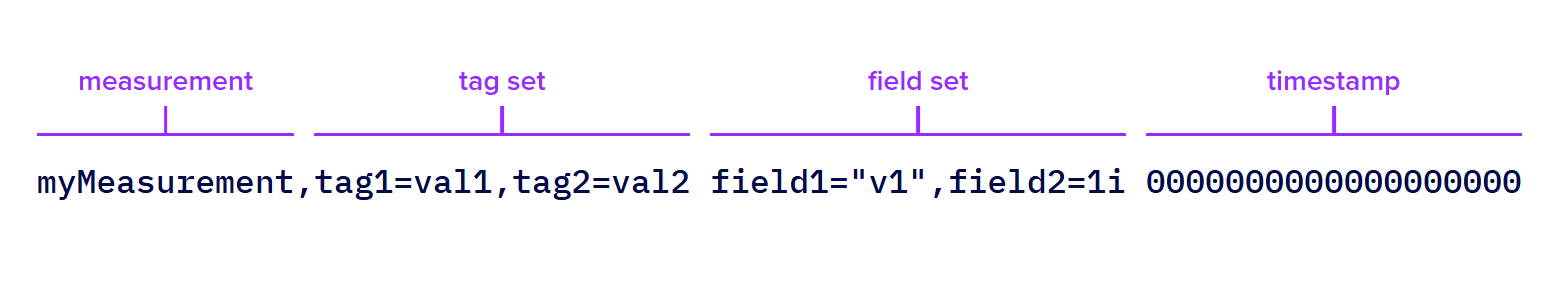
\includegraphics[width=0.85\textwidth]{figures/line_protocol.png} 
    \caption{Az InfluxDB Line Protocol felépítése}
    \label{fig:line_protocol}
\end{figure}

A formátumot alkotó szintaktikai elemek szemantikai jelentése és szerepe az idősor-alapú (\textit{Time Series}) adatmodellezésben a következő:

\begin{itemize}
    \item \textbf{Measurement (Mérés):} A relációs adatbázisok táblaneveivel analóg strukturális elem (a rendszerben ilyen például a \texttt{death} mérés). Ez határozza meg a rögzíteni kívánt esemény vagy metrika alapvető kontextusát.

    \item \textbf{Tag-ek (Címkék):} Kulcs-érték párok formájában megadott metaadatok, amelyeket az InfluxDB \textbf{automatikusan indexel}. Mivel az indexelés miatt ezeken a mezőkön a lekérdezések futási ideje konstans vagy logaritmikus, ide a diszkrét, kategorizálható tulajdonságokat (például \texttt{species}, \texttt{cause}, \texttt{run\_id}) érdemes helyezni. Fontos tervezési szabály, hogy a tag-ek értékei sztring típusúak, és nem tartalmazhatnak nagy kardinalitású, folyamatosan változó értékeket (példánkban a futás azonosítója fix a szimuláció alatt).

    \item \textbf{Field-ek (Mezők):} Kulcs-érték párok, amelyek a szimuláció \textbf{ténylegesen mért, változó célértékeit} (metrikáit) hordozzák (például \texttt{speed}, \texttt{sight}, \texttt{age}). A mezők értékei nem indexeltek, de rajtuk matematikai és statisztikai aggregációk (átlagolás, minimum- és maximumkeresés, integrálás) végezhetők. Értékük lehet lebegőpontos szám, egész szám, logikai érték vagy sztring.

    \item \textbf{Timestamp (Időbélyeg):} Az esemény bekövetkezésének pontos ideje. Mivel az URL-ben a \texttt{precision=s} paramétert használjuk, ez másodperc alapú UNIX időbélyegként értelmeződik. Ha nincs explicit módon megadva, az InfluxDB a kérés szerverre érkezésének pillanatát rendeli hozzá a ponthoz.
\end{itemize}

A szintaxis szempontjából kritikus pont a \textbf{szóköz karakterek} elhelyezkedése: az első szóköz választja el az indexelt metaadatokat (Measurement és Tag-ek) a nem indexelt értékektől (Field-ek), míg a második szóköz különíti el a mezőket a záró időbélyegtől. A Tag-ek és Field-ek listáján belüli elemeket vesszővel (\texttt{,}) kell elválasztani, a kulcs-érték párokat pedig egyenlőségjellel (\texttt{=}), szóközök nélkül.

A \texttt{DebugLogger.RegisterDeathToDb} metódus az egyedek pusztulásakor pontosan ebben a struktúrában állítja össze a telemetriai csomagot. A hatékony lekérdezhetőség érdekében a fix tulajdonságokat (faj, halál oka, szimulációs futás azonosítója...) \textit{Tag}-ként, míg a folyamatosan változó, mutációra képes genetikai és viselkedési attribútumokat \textit{Field}-ként definiálja a rendszer.

Egy elpusztult nyúl (Bunny) adatainak felküldésekor generált Line Protocol sztring felépítése (a hiba elkerülése végett nyelvi kiemelés nélkül):

\begin{lstlisting}[caption={Példa InfluxDB Line Protocol formátumú üzenetre}]
death,run_id=20260527_224700,species=BUNNY,cause=CONSUMED age=1.2,speed=5.4,sight=15.0,
lifeSpan=60.0,charm=42.0,pregnancyDuration=10.0,starving=30.0,drying=40.0,triedForBaby=2,
gaveBirth=0,kids=0,step=1420
\end{lstlisting}

A formátum kulcsfontosságú elemei a szimuláció szempontjából:
\begin{itemize}
    \item \textbf{Measurement (\texttt{death}):} az esemény típusa (idősor-tábla neve)
    \item \textbf{Tags (\texttt{run\_id}, \texttt{species}, \texttt{cause}):} indexelt metaadatok

Ezek alapján a Grafana felületén rendkívül gyorsan lehet szűrni az adatokat (pl. külön vizualizálni a rókák és a nyulak halálozási okait).
    \item \textbf{Fields (pl. \texttt{speed}, \texttt{sight}, \texttt{step}):} nem indexelt értékek

Ezek hordozzák a populáció aktuális átlagértékeit, amelyekből a statisztikai trendek, az evolúciós növekedés vagy a természetes szelekció iránya számszerűsíthető.
\end{itemize}

Az így kiküldött adatok közvetlenül az InfluxDB \texttt{bucket}-jébe\footnote{Az InfluxDB kontextusában a \textit{bucket} egy logikai adattároló egység (analóg a relációs adatbázisok adatbázis-fogalmával), amely meghatározott adatmegőrzési szabályokkal (\textit{Retention Policy}) rendelkezik, és idősoros adatok (\textit{time series data}) strukturált tárolására szolgál.} kerülnek, ahonnan a Grafana dashboardok valós időben, másodperces felbontással képesek kirajzolni a populáció túlélési és adaptációs grafikonjait.